\documentclass[tikz,border=2pt]{standalone}
\usepackage{amsmath,amssymb}
\usepackage{tikz}

\begin{document}
% Two fair dice: F(2, 3) adds the masses of the 6 outcomes with x <= 2 and y <= 3.
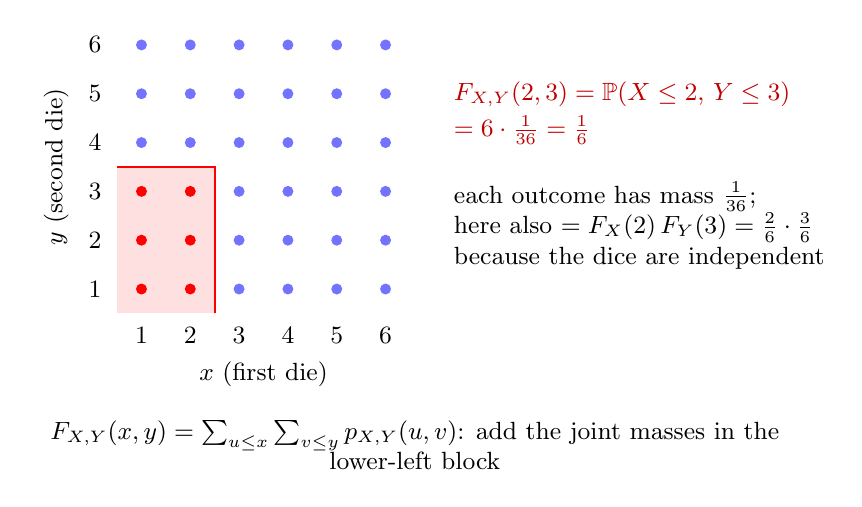
\begin{tikzpicture}[every node/.style={font=\small}, scale=0.62]
	\fill[red!12] (0.5,0.5) rectangle (2.5,3.5);
	\draw[red, thick] (2.5,0.5) -- (2.5,3.5) -- (0.5,3.5);
	\foreach \x in {1,...,6} {
		\foreach \y in {1,...,6} {
			\pgfmathtruncatemacro{\inside}{(\x<3 && \y<4) ? 1 : 0}
			\ifnum\inside=1
				\fill[red] (\x,\y) circle (3.2pt);
			\else
				\fill[blue!55] (\x,\y) circle (3.2pt);
			\fi
		}
		\node[font=\small] at (\x,0.05) {$\x$};
		\node[font=\small] at (0.05,\x) {$\x$};
	}
	\node[font=\small] at (3.5,-0.75) {$x$ (first die)};
	\node[font=\small, rotate=90] at (-0.75,3.5) {$y$ (second die)};
	\node[red!75!black, anchor=west, align=left] at (7.2,4.6) {$F_{X,Y}(2,3)=\mathbb{P}(X\le2,\,Y\le3)$\\[2pt] $=6\cdot\tfrac1{36}=\tfrac16$};
	\node[anchor=west, align=left, font=\small] at (7.2,2.3) {each outcome has mass $\tfrac1{36}$;\\ here also $=F_X(2)\,F_Y(3)=\tfrac26\cdot\tfrac36$\\ because the dice are independent};
	\node[anchor=north, align=flush center, text width=9.6cm] at (6.6,-1.5) {$F_{X,Y}(x,y)=\sum_{u\le x}\sum_{v\le y}p_{X,Y}(u,v)$: add the joint masses in the lower-left block};
\end{tikzpicture}
\end{document}
